\chapter{Testabdeckung}
\section{App}
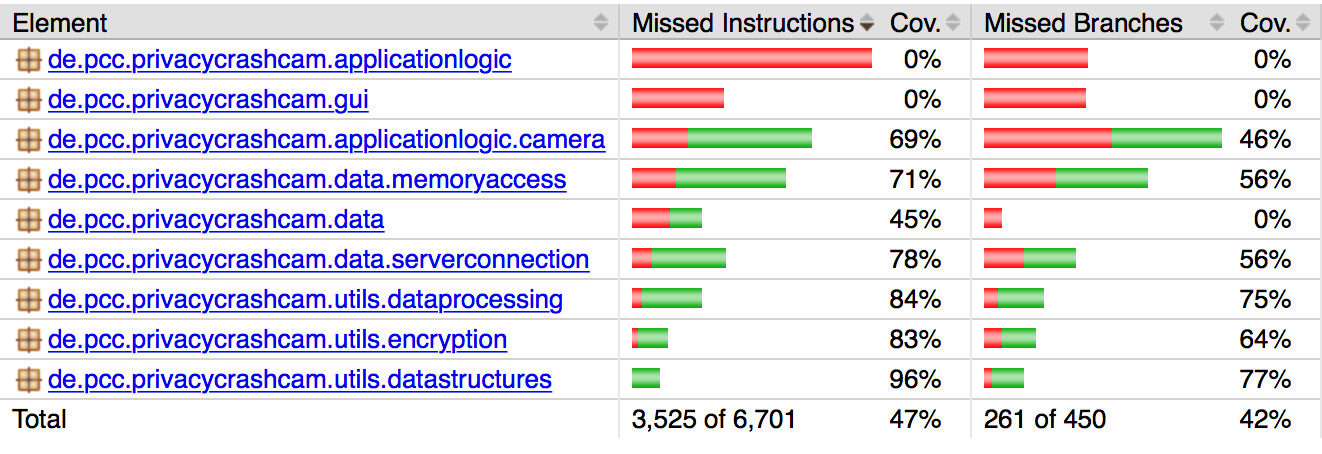
\includegraphics[scale=0.6]{resources/coverage/app/Coverage.jpg}
Die Testabdeckung in der App festzustellen hat sich schon früh als problematisch herausgestellt. Durch zahlreiche Abhängigkeiten zu Klassen des Android Frameworks ist es nicht immer möglich, Stubs oder Mocks aller Abhängigkeiten anzubieten und so können die betroffenen Funktionen nicht getestet werden. Da die UI-Tests ebenfalls nicht automatisiert ablaufen erscheint somit die resultierende Testabdeckung als gering. Hier darf nicht die begrenzte Aussagekraft der Testüberdeckung vergessen werden, denn bei genauerem Hinsehen wurden Kern-Funktionen so gut es Android zulässt abgedeckt. In der obigen Grafik ist die Testüberdeckung der Module zu sehen.

\section{Webinterface}
Die Funktionalität der Datenmanagerklassen sind mit automatisierten Tests gedeckt. Dadurch wird im Webinterface jedoch nur eine geringe Testüberdeckung durch automatisierte Tests erreicht. Deshalb wurden manuelle Tests, zum Testen der Funktionalität der graphischen Benutzeroberfläche durchgeführt, um eine höhere Überdeckung zu gewährleisten.

\section{Webservice}
\subsection{data}
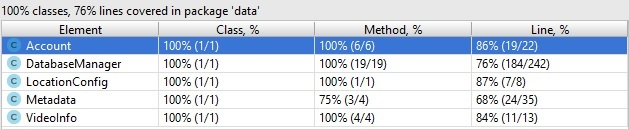
\includegraphics[scale=0.8]{resources/data.jpg}
Das data-packge beinhaltet die verschiedenen Datenklassen, die Accountdaten sowie Video und Metainformationen beinhalten. Die Testüberdeckung in diesen Klassen geschieht größtenteils durch Tests in anderen packages (Server/Manager Module). Die relevanteste Klasse innerhalb dieses Moduls ist der DatabaseManager. Dieser wurde ausgiebig getestet und überdeckt einen großen Teil der anderen  Klassen.
\subsection{manager}
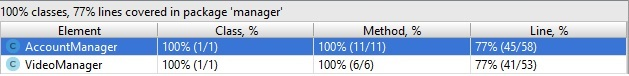
\includegraphics[scale=0.8]{resources/manager.jpg}
Das manager-package beinhaltet den VideoManager und den AccountManager. Die beiden Tests überdecken den größten Teil beider Klassen. Durch den ServerProxyTest wird nebenbei auch noch ein großer Teil der beiden Manager überdeckt. Der Fokus der Tests lag darauf korrekte Ergebnisse bei korrekten Parametern zu erlangen.
\subsection{server}
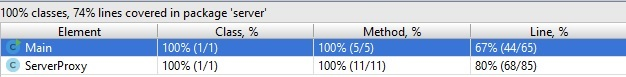
\includegraphics[scale=0.81]{resources/server.jpg}
Das service-package beinhaltet den ServerProxy und die Main-Klasse, die in großem Format durch den ServerProxyTest überdeckt sind. Dieser ist Integrations- sowie Komponententest in einem. Der Fokus lag dabei die Rest-Schnittstelle anzusprechen und durch verschiedene Daten und Accounts die Korrektheit der Ergebnisse des ServerProxy zu überprüfen. 
\subsection{videoprocessing}
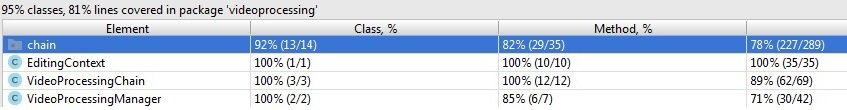
\includegraphics[scale=0.6]{resources/videoprocessing.jpg}
Das videoprocessing-package beinhaltet die komplette Funktion das Video zu bearbeiten (entschlüsseln, anonymisieren, persistieren). Dabei wurde während des Testens Fokus darauf gelegt, das die komplette Funktionalität sowohl mit korrekten als auch mit fehlerhaften Daten zum gewünschten Ergebnis. 

\section{Bewertung}
Unter Beachtung der oben genannten Probleme und Schwierigkeiten, die das Erreichen einer 100\%igen Testüberdeckung erschweren, sichern unsere Tests Kernfunktionalitäten, die in Model und Controller implementiert sind. Die größten Defizite ergeben sich bei UI-Klassen. Deren Funktionalität konnten wir jedoch anhand unserer Testprotokolle abdecken.